\chapter{TỔNG QUAN}
\label{chap:chap1-introduce}
\nocite{*}
Trong chương này, tác giả sẽ giới thiệu về đề tài, trình bày lý do chọn đề tài, mục tiêu nghiên cứu, đối tượng và phạm vi nghiên cứu.

\section{Đặt vấn đề}
\subsection{Giới thiệu đề tài}
Trong thời đại công nghệ số, cùng với sự phát triển của trí tuệ nhân tạo và học sâu, việc xây dựng các hệ thống có khả năng hiểu và tương tác với thông tin đa phương tiện trở thành một xu hướng tất yếu. Bên cạnh văn bản và âm thanh, hình ảnh đóng vai trò quan trọng trong việc truyền tải thông tin phong phú và trực quan. Tuy nhiên, để máy tính có thể hiểu và trả lời các câu hỏi liên quan đến hình ảnh là một thách thức lớn, đòi hỏi sự kết hợp chặt chẽ giữa xử lý ngôn ngữ tự nhiên và thị giác máy tính. Bài toán Hỏi đáp hình ảnh (Visual Question Answering – VQA) đã ra đời nhằm giải quyết vấn đề này, cho phép hệ thống không chỉ nhận diện nội dung trong ảnh mà còn suy luận để đưa ra câu trả lời phù hợp cho câu hỏi được đặt ra.

Trong bối cảnh đó, một hướng tiếp cận quan trọng và thực tế là tập trung vào các câu hỏi dạng Yes/No. Thay vì phải sinh ra câu trả lời tự do hoặc chọn từ một tập hợp rộng các đáp án, hệ thống chỉ cần dự đoán giữa hai khả năng có/không, đúng/sai. Điều này giúp đơn giản hóa bài toán, đồng thời tạo nền tảng để phát triển các ứng dụng trong đời sống như trợ lý ảo cho người khiếm thị, hệ thống kiểm chứng thông tin hình ảnh, hay các ứng dụng hỗ trợ giáo dục trực quan.

Bài toán Hỏi đáp hình ảnh với câu hỏi Yes/No bằng mô hình CLIP ra đời như một giải pháp hiệu quả, tận dụng sức mạnh của mô hình ngôn ngữ – hình ảnh đã được huấn luyện trên lượng dữ liệu khổng lồ. Thay vì huấn luyện lại từ đầu, việc khai thác CLIP giúp hệ thống có khả năng liên kết ngữ nghĩa giữa văn bản và hình ảnh một cách mạnh mẽ, từ đó đưa ra câu trả lời Yes/No chính xác hơn. Vì vậy, trong khóa luận này, chúng tôi tập trung nghiên cứu và đánh giá hiệu quả của mô hình CLIP trong bài toán Hỏi đáp hình ảnh dạng Yes/No, với đầu vào là cặp (ảnh, câu hỏi) và đầu ra là câu trả lời nhị phân tương ứng. 

\vspace{0.5cm}
\[
\begin{array}{ll}
\textbf{Tập dữ liệu:} & \mathcal{D} = \{(x_i, q_i, y_i)\}_{i=1}^N \\[1em]

\textbf{Input:} &
\left\{
\begin{array}{ll}
x \in \mathbb{R}^{H \times W \times C}, & \text{Ảnh đầu vào} \\[2pt]
q = (w_1, w_2, \dots, w_T),\; \mathbf{q} \in \mathbb{R}^{d_q}, & \text{Câu hỏi Y/N ?} \\[2pt]
\mathcal{L} = \{\text{Yes}, \text{No}\} & \text{Tập nhãn có thể có}
\end{array}
\right. \\[1em]

\textbf{Output:} & \hat{y} = f(x, q) \in \mathcal{L}, \quad \text{Nhãn dự đoán}
\end{array}
\]
\vspace{0.5cm}

\begin{figure}[!hbt]
    \centering
    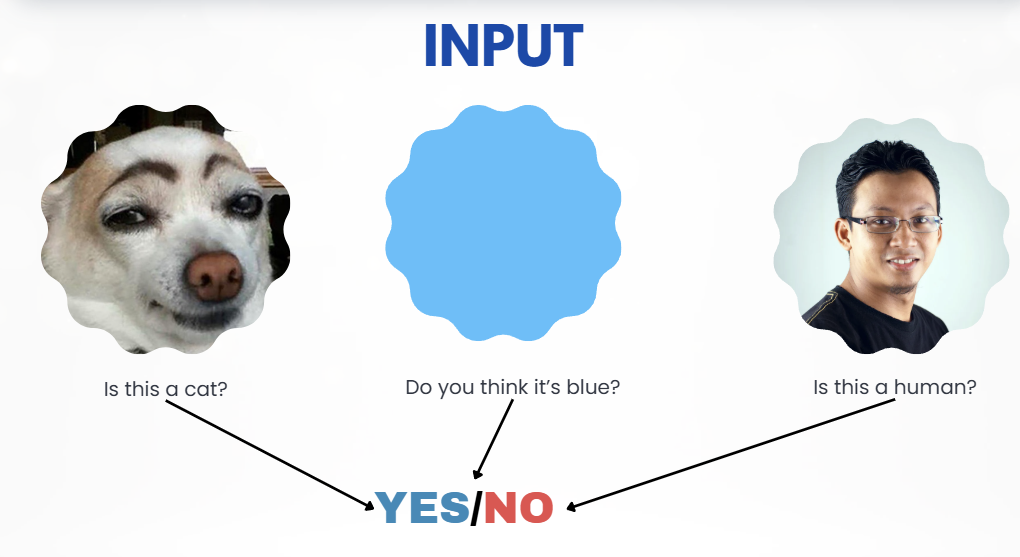
\includegraphics[width=0.85\linewidth]{graphics/chapter1/minhhoa.png}
    \caption{Hình ảnh minh họa cho bài toán}
    \label{fig:MH1}
\end{figure}


\subsection{Lý do chọn đề tài}

Trong bối cảnh trí tuệ nhân tạo và thị giác máy tính phát triển nhanh chóng, việc xây dựng các hệ thống có khả năng hiểu và trả lời câu hỏi dựa trên hình ảnh (Visual Question Answering - VQA) ngày càng trở nên quan trọng và mang tính ứng dụng cao. Trong lĩnh vực hỗ trợ người khiếm thị, VQA giúp họ có thể đặt câu hỏi về hình ảnh xung quanh để nhận thông tin cần thiết. Trong giáo dục, công nghệ này hỗ trợ xây dựng các hệ thống học tập thông minh, giúp học sinh có thể hỏi và nhận câu trả lời trực quan từ hình ảnh. Trong thương mại điện tử và truyền thông, VQA giúp tăng cường trải nghiệm người dùng thông qua việc tìm kiếm và gợi ý sản phẩm dựa trên hình ảnh đi kèm câu hỏi.

Để hiện thực hóa các ứng dụng đó, các mô hình VQA cần có khả năng không chỉ nhận diện đối tượng trong ảnh mà còn phải kết hợp thông tin từ cả hình ảnh và câu hỏi văn bản để suy luận chính xác. Trong đó, dạng câu hỏi Yes/No là một trong những loại câu hỏi phổ biến và cơ bản nhất, đóng vai trò nền tảng cho việc phát triển các hệ thống VQA phức tạp hơn. Giải quyết bài toán này cũng góp phần hướng đến việc tham gia và thử nghiệm trên các bộ dữ liệu thách thức trong lĩnh vực VQA, tiêu biểu như \href{https://vizwiz.org/tasks-and-datasets/vqa/}{VizWiz VQA Challenge}.

Kho lưu trữ mã nguồn mở \href{https://github.com/yousefkotp/Visual-Question-Answering?tab=readme-ov-file}{Visual
 Question Answering with CLIP} cung cấp nền tảng nghiên cứu và thực nghiệm quan trọng cho đề tài này. Dựa trên đó, đề tài tập trung vào việc xây dựng và đánh giá mô hình Hỏi đáp hình ảnh với câu hỏi Yes/No, nhằm khai thác sức mạnh của mô hình CLIP trong việc liên kết ngôn ngữ và thị giác, mở ra nhiều hướng ứng dụng thực tiễn trong đời sống.
\section{Mục tiêu nghiên cứu}

Trong quá trình giao tiếp và khai thác thông tin từ hình ảnh, con người thường đặt ra những câu hỏi ngắn gọn, đơn giản nhưng mang tính thiết yếu, điển hình là dạng câu hỏi \textit{Yes/No}. Những câu hỏi này không chỉ giúp xác định sự hiện diện hay đặc điểm của đối tượng trong ảnh mà còn thể hiện nhu cầu tiếp cận thông tin nhanh, rõ ràng và trực quan. Chính vì vậy, việc xây dựng hệ thống có khả năng tự động trả lời các câu hỏi Yes/No từ hình ảnh không chỉ là một hướng nghiên cứu quan trọng trong lĩnh vực Thị giác máy tính và Ngôn ngữ tự nhiên mà còn có ý nghĩa ứng dụng thực tiễn trong nhiều lĩnh vực như hỗ trợ người khiếm thị, giáo dục, thương mại điện tử hay các hệ thống trợ lý thông minh.

Trong nghiên cứu này, chúng tôi tập trung vào việc khai thác sức mạnh của mô hình CLIP để xây dựng hệ thống hỏi đáp hình ảnh cho dạng câu hỏi Yes/No. Cụ thể, đề tài tập trung vào các mục tiêu sau:

\begin{enumerate}
\item Tìm hiểu tổng quan về bài toán Visual Question Answering (VQA), đặc biệt là dạng câu hỏi Yes/No, nhằm nắm vững cơ sở lý thuyết và những thách thức chính của bài toán.
\item Nghiên cứu các phương pháp tiếp cận đã có trong lĩnh vực VQA, phân tích ưu nhược điểm của từng hướng để lựa chọn chiến lược áp dụng phù hợp cho bài toán.
\item Xây dựng và xử lý tập dữ liệu phù hợp cho dạng câu hỏi Yes/No, đảm bảo dữ liệu có tính đa dạng và phản ánh đúng các tình huống thường gặp.
\item Khai thác mô hình CLIP trong việc kết hợp thông tin hình ảnh và văn bản, đồng thời nghiên cứu các kỹ thuật tinh chỉnh (fine-tuning) để tối ưu khả năng suy luận Yes/No.
\item Triển khai, đánh giá và so sánh hiệu suất mô hình trên các tập dữ liệu chuẩn trong lĩnh vực VQA. Việc đánh giá tập trung vào các tiêu chí như độ chính xác trong câu trả lời, khả năng khái quát hóa và độ tin cậy khi áp dụng vào thực tế.
\end{enumerate}

\subsection{Thách thức và giải pháp}

\begin{enumerate}
    \item \textbf{Hiểu ngữ cảnh giữa ảnh và câu hỏi (Cross-modal reasoning)} 
    
    Câu hỏi Yes/No đôi khi cần suy luận ngữ cảnh, không chỉ là khớp trực tiếp ảnh – ví dụ: 
    
    \textit{“Có phải đây là cánh cửa đang mở không?”}
    
    Trong trường hợp này, mô hình không chỉ cần nhận diện đối tượng \textit{cánh cửa}, mà còn phải hiểu trạng thái của nó (\textit{đang mở}) để đưa ra câu trả lời chính xác. Điều này đòi hỏi khả năng suy luận đa phương thức (cross-modal reasoning) giữa ảnh và ngôn ngữ, vốn là một thách thức khó trong các mô hình thị giác-ngôn ngữ hiện nay. 
    
    \textbf{Giải pháp:} Bổ sung thêm \textit{knowledge distillation} từ các mô hình ngôn ngữ lớn (LLM) để tăng khả năng suy luận ngữ cảnh. Việc này giúp mô hình học được kiến thức ngôn ngữ phong phú từ LLM, từ đó cải thiện khả năng kết nối ngữ nghĩa giữa câu hỏi và hình ảnh.

    \item \textbf{Hiệu suất mô hình CLIP chưa tối ưu cho Yes/No Question} \\
    Mô hình CLIP vốn được huấn luyện cho nhiệm vụ so khớp ảnh -- văn bản tổng quát, chưa được tinh chỉnh chuyên biệt cho các câu hỏi dạng Yes/No. Điều này dẫn đến việc phân biệt ranh giới giữa hai nhãn \textit{Yes} và \textit{No} còn hạn chế. \\ 
    \textbf{Giải pháp:} Áp dụng \textit{contrastive learning} bổ sung: xây dựng cặp (ảnh, câu hỏi đúng) và (ảnh, câu hỏi nhiễu) để mô hình học cách phân biệt tốt hơn, từ đó cải thiện khả năng dự đoán Yes/No.
\end{enumerate}




Thông qua việc ứng dụng mô hình CLIP vào dạng câu hỏi Yes/No, đề tài kỳ vọng đóng góp một giải pháp hiệu quả, nhẹ và có khả năng mở rộng, làm nền tảng cho việc phát triển các hệ thống VQA thông minh, dễ triển khai trong thực tiễn.
\section{Phạm vi - Đối tượng nghiên cứu}

\subsection{Phạm vi nghiên cứu}

Bài toán là một trong các nhiệm vụ cần giải quyết của thử thách \textit{Visual Question Answering (VQA)} trên bộ dữ liệu \textbf{VizWiz-VQA}. 
Ở thử thách \textit{VQA dạng Yes/No question}, cho một bức ảnh do người khiếm thị chụp và một câu hỏi tương ứng, hệ thống được yêu cầu đưa ra câu trả lời nhị phân ``Yes'' hoặc ``No'' dựa trên nội dung ảnh. 
Câu hỏi có thể liên quan trực tiếp đến sự hiện diện, đặc điểm hoặc hành động của đối tượng trong ảnh. 
Đặc thù của VizWiz-VQA là nhiều ảnh có chất lượng thấp (mờ, thiếu sáng, bố cục không rõ ràng) và câu hỏi có thể \textit{không thể trả lời được (unanswerable)}, từ đó làm tăng tính thách thức cho mô hình. 
Đây là dạng câu hỏi trắc nghiệm nhị phân, chỉ có một đáp án đúng cho mỗi trường hợp.  

\begin{figure}[!hbt]
    \centering
    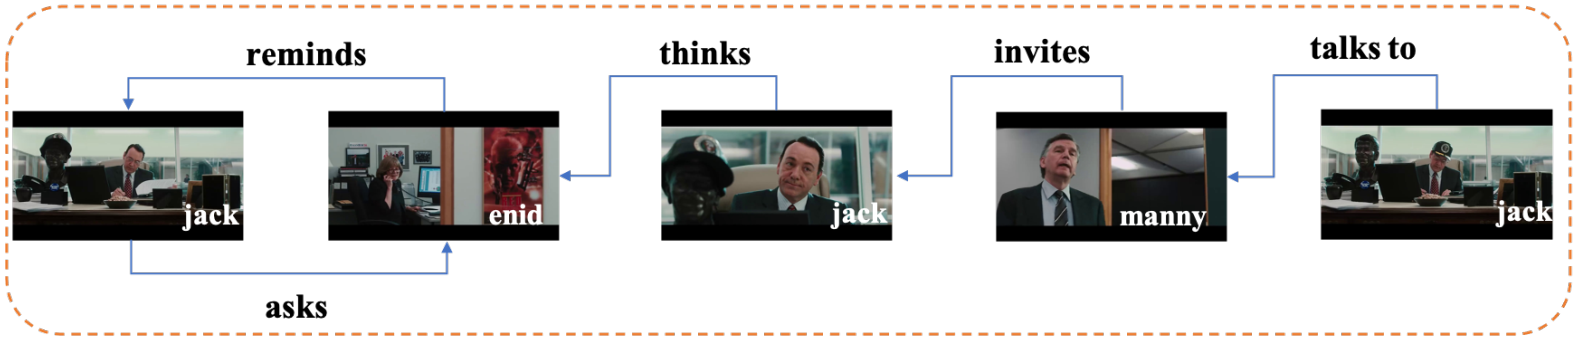
\includegraphics[width=1.0\linewidth]{graphics/chapter1/next_previous_in.png}
    \caption{Hình ảnh minh họa cho next or previous interaction}
\end{figure}

Bộ dữ liệu \textbf{VizWiz-VQA} cung cấp các mẫu câu hỏi thực tế kèm theo đáp án từ nhiều người gán nhãn, trong đó có một tập lớn câu hỏi dạng Yes/No. 
Dựa vào đó, chúng tôi định hướng nghiên cứu khóa luận này trong phạm vi \textbf{bài toán VQA dạng Yes/No}, nhằm xây dựng một bộ dữ liệu con cụ thể phục vụ cho nghiên cứu và đánh giá hiệu quả của mô hình.  

\begin{figure}[!hbt]
    \centering
    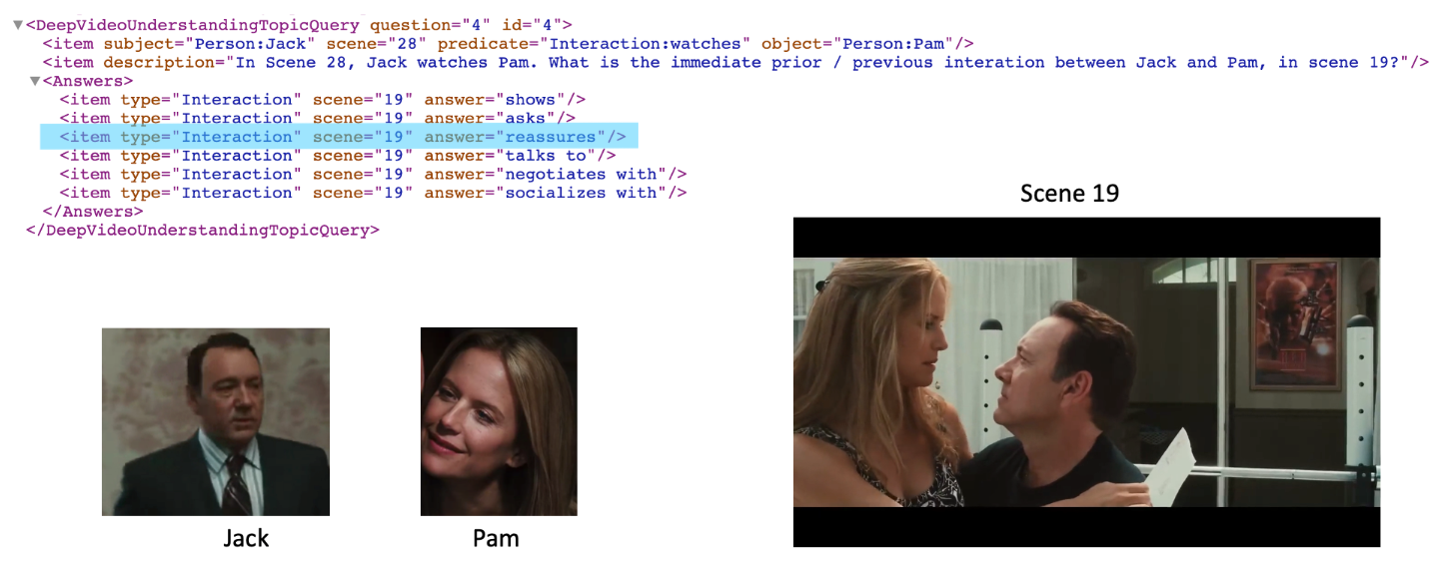
\includegraphics[width=1.0\linewidth]{graphics/chapter1/next_previous_in1.png}
    \caption{Mẫu câu hỏi ở cấp độ cảnh quay cho Find next or previous interaction}
    \label{fig:next_previous}
\end{figure}

\subsection{Xây dựng bộ dữ liệu}
Về việc xây dựng bộ dữ liệu, chúng tôi tập trung lọc và chuẩn hóa các cặp \textit{(ảnh, câu hỏi, nhãn Yes/No)} từ VizWiz-VQA, 
đồng thời đề xuất phương pháp xử lý các trường hợp \textit{unanswerable} để đảm bảo chất lượng bộ dữ liệu cho bài toán phân loại nhị phân.  

\subsection{Phương pháp nghiên cứu}
Về phương pháp, khóa luận chủ yếu xoay quanh việc áp dụng mô hình \textbf{CLIP (Contrastive Language--Image Pretraining)} cho nhiệm vụ VQA dạng Yes/No. 
CLIP cho phép học biểu diễn kết hợp từ hai loại dữ liệu đầu vào: \textit{ảnh} và \textit{văn bản câu hỏi}, từ đó khai thác đặc trưng liên kết giữa nội dung hình ảnh và ngôn ngữ tự nhiên. 
Đề tài tập trung vào việc nghiên cứu và đề xuất các cách \textit{fine-tune CLIP} hoặc kết hợp thêm tầng phân loại để tối ưu hiệu quả trong bài toán Yes/No trên VizWiz-VQA.


\subsection{Đối tượng nghiên cứu}
\begin{enumerate}
    \item \textbf{Đối tượng nghiên cứu thứ nhất} của đề tài này là các câu hỏi dạng Yes/No trong bộ dữ liệu VizWiz-VQA. 
    Cụ thể, chúng tôi chọn tập con các câu hỏi Yes/No bởi đây là loại câu hỏi phổ biến, có ý nghĩa thực tiễn và phù hợp với phạm vi nghiên cứu. 
    Việc tập trung vào câu hỏi Yes/No giúp giới hạn độ phức tạp, đồng thời vẫn đảm bảo đủ thách thức do đặc thù của VizWiz-VQA là ảnh thường có chất lượng thấp và câu hỏi có thể không thể trả lời được.  

    \item \textbf{Đối tượng nghiên cứu thứ hai} là quá trình xử lý và gán nhãn dữ liệu. 
    Bộ dữ liệu VizWiz-VQA ở dạng gốc chứa nhiều loại câu hỏi khác nhau, do đó cần tiến hành lọc và chuẩn hóa thành tập dữ liệu chỉ gồm \textit{(ảnh, câu hỏi Yes/No, nhãn Yes/No)}. 
    Ngoài ra, việc xử lý các trường hợp \textit{unanswerable} cũng được chú trọng để đảm bảo tính nhất quán và độ tin cậy của dữ liệu đầu vào.  

    \item \textbf{Đối tượng nghiên cứu thứ ba} là tìm hiểu và áp dụng mô hình trích xuất đặc trưng từ dữ liệu đa phương thức (multimodal). 
    Trong bài toán này, hai loại dữ liệu đầu vào là \textit{ảnh} và \textit{câu hỏi văn bản}. 
    Việc khai thác đặc trưng từ ảnh và văn bản, cũng như ánh xạ chúng vào cùng một không gian biểu diễn, là trọng tâm để mô hình có thể suy luận chính xác trong các câu hỏi Yes/No.  

    \item \textbf{Đối tượng nghiên cứu cuối cùng} là mô hình phân loại Yes/No dựa trên đặc trưng đầu vào và đánh giá kết quả. 
    Cụ thể, chúng tôi sử dụng mô hình \textbf{CLIP (Contrastive Language--Image Pretraining)} làm nền tảng, sau đó thử nghiệm các cách fine-tune hoặc bổ sung tầng phân loại để tối ưu hiệu quả. 
    Mô hình có kết quả tốt nhất sẽ được chọn làm minh họa cho khả năng áp dụng CLIP trong bài toán VQA dạng Yes/No trên VizWiz-VQA.  
\end{enumerate}

\section{Đóng góp của đồ án}
Khi hoàn thành, đồ án mang lại những đóng góp:

\begin{itemize}
    \item Hệ thống lại các hướng tiếp cận trong lĩnh vực Visual Question Answering (VQA), đặc biệt với dạng câu hỏi Yes/No và các thách thức của bộ dữ liệu VizWiz-VQA.
    \item Cung cấp kiến thức nền tảng về mô hình \textbf{CLIP}, cơ chế học biểu diễn kết hợp ngôn ngữ--hình ảnh, cùng các phương pháp fine-tuning trong học sâu.
    \item Đề xuất và triển khai phương pháp gán nhãn cho các câu hỏi khó hoặc không trả lời được (\textit{unanswerable}), nhằm đảm bảo tính toàn vẹn và chất lượng của tập dữ liệu.
    \item Xây dựng pipeline tiền xử lý dữ liệu gồm chuẩn hóa câu hỏi, xử lý ảnh đầu vào và tổ chức dữ liệu cho bài toán phân loại Yes/No.
    \item Cài đặt thực nghiệm mô hình CLIP với nhiều cấu hình khác nhau, tiến hành so sánh và đánh giá hiệu quả mô hình trên bộ dữ liệu VizWiz-VQA.
    \item Làm cơ sở để mở rộng nghiên cứu sang các loại câu hỏi khác trong VQA hoặc áp dụng cho các bài toán multimodal trong thực tế.
\end{itemize}






